\subsection{ASGAL}
ASGAL (Alternative Splicing Graph Aligner) è un tool per l'identificazione di eventi di Alternative Splicing espressi in un campione di RNA-seq a partire
da un'annotazione di un gene. ASGAL si compone di tre step:

\begin{itemize}
	\item Costruzione dello splicing graph: a partire dall'annotazione di un gene, ASGAL costruisce uno splicing graph\footnote{Uno splicing graph è una struttura a grafo che...} che rappresenta la struttura del gene a partire dai trascritti dati in input
	\item Allineamento Splice-Aware\footnote{Splice-Aware significa che...}: ASGAL allinea le read di RNA-Seq con lo splicing graph del gene in input.
	\item Rilevamento degli eventi di Alternative Splicing: gli allineamenti prodotti dallo step precedente sono analizzati per rilevare gli eventi di alternative splicing indotti dalle read del campione.
\end{itemize}

\begin{figure}[b!]
	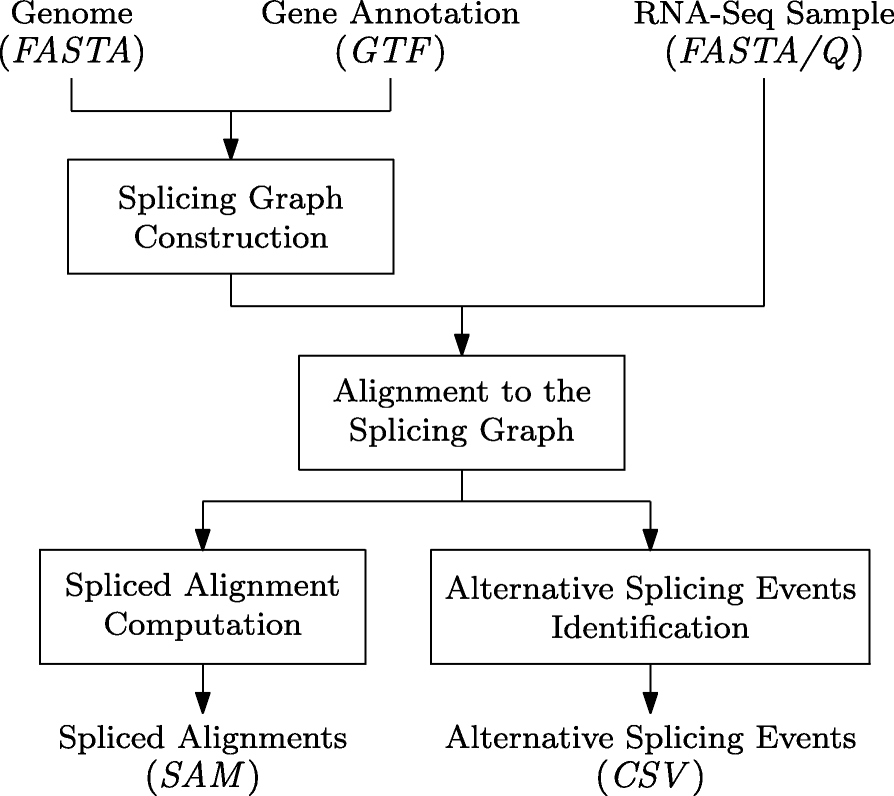
\includegraphics[width=\linewidth]{images/asgal.png}
  \caption{La pipeline di ASGAL illustrata}
  \label{fig:ASGAL}
\end{figure}